\section{\Grappa Overview}

% Commodity clusters provide fast processors and high-bandwidth
% interconnects but suffer when they encounter unpredictable data access
% patterns. Maximizing throughput in such a situation depends upon
% proper management of concurrency and communication. 

\Grappa's design is motivated by two key observations of today's systems.
First, modern compute cores can execute hundreds of thousands of instructions
in the few microseconds that it takes for one remote memory read to complete. Second,
the injection rate of modern commodity networks is low and the bandwidth is
optimized for large messages. Given the frequent communication caused by high
degree of fine-grained random access in irregular applications, it is
necessary to both overlap communication with computation as much as possible
and to aggregate network messages efficiently. Providing these two properties
depend on exploiting large amounts of concurrency. Hence, \Grappa's
programming model focuses on enabling programmers to easily express
concurrency.

% \Grappa is intended to support what we
% think is a desirable workflow: programmers start by expressing a computation
% using a multithreaded, shared-memory model on a single node. \Grappa then
% provides the primitives to do a straightforward translation of this code to
% run on a distributed-memory cluster, through constructs for optimizing
% locality and overlapping communication.

\Grappa comprises three main software components, shown in Figure~\ref{fig:grappa}:

\begin{figure}[t]
\begin{center}
  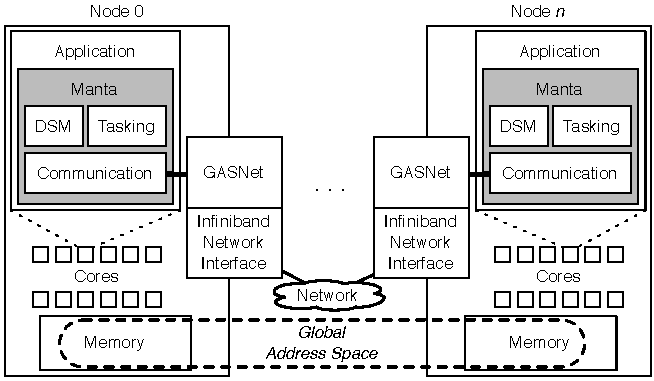
\includegraphics[width=0.95\columnwidth]{figs/system-overview}
\begin{minipage}{0.95\columnwidth}
  \caption{\label{fig:grappa} \Grappa system overview}
\end{minipage}
\vspace{-3ex}
\end{center}
\end{figure}

\begin{description}

\item [Tasking system] The tasking system supports lightweight multithreading
to tolerate communication latency and global distributed work-stealing (i.e.,
tasks can be stolen from any node in the system), which provides automated
load balancing. The scheduler oversubscribes to have more worker threads than
required for latency tolerance. By keeping at least four workers per 
core ready to run at all times, the scheduler can prefetch a worker's state
into cache to reduce the chance of stalling on memory accesses during a
context switch.

\item[Communication layer] The main goal of our communication layer is to
aggregate small messages into large ones. This process is invisible to the
application programmer. Its interface is based on active
messages~\cite{vonEicken92}. Since aggregation and deaggregation of messages
needs to be very efficient, we perform the process in parallel and carefully
use lock-free synchronization operations. 

GASNet~\cite{gasnet} is used as the
underlying mechanism for bulk remote memory reads and writes using active message
invocations, with an off-the-shelf user-mode InfiniBand device driver
stack~\cite{OFED}. MPI is used for process setup and tear down.


\item[Distributed shared memory] The DSM system provides fine-grain access to
data anywhere in the system, with delegated operation at the core of its design.
Every piece of global memory is owned by a particular core in the system, and all others may only access that memory by delegating their requests to the owning core.
It supports normal access operations such as
\emph{read\/} and \emph{write\/} as well as synchronizing operations such as
\emph{fetch-and-add\/}~\cite{fetchandadd}. Due to delegation, the memory model offered is similar to what underpins
C/C++~\cite{N2480,N2800}, so it is familiar to programmers. The DSM system
design relies on the lightweight tasking system and communication layer in
order to offer high aggregate random access bandwidth for accessing remote
data.

\end{description}

% \Grappa leverages as much freely available and commodity infrastructure as
% possible. We use unmodified Linux for the operating system and an
% off-the-shelf user-mode InfiniBand device driver stack~\cite{OFED}. MPI is
% used for process setup and tear down. GASNet~\cite{gasnet} is used as the
% underlying mechanism for remote memory reads and writes using active message
% invocations.
